\documentclass{beamer}
%\usepackage[margin=1in]{geometry}
\usepackage{amsthm,amsmath,amsfonts,hyperref,graphicx,color,multicol}
\usepackage{enumitem,tikz}

%%%%%%%%%%
%Beamer Template Customization
%%%%%%%%%%
\setbeamertemplate{navigation symbols}{}
\setbeamertemplate{theorems}[ams style]
\setbeamertemplate{blocks}[rounded]

\definecolor{Blu}{RGB}{43,62,133} % UWEC Blue
\setbeamercolor{structure}{fg=Blu} % Titles

%Unnumbered footnotes:
\newcommand{\blfootnote}[1]{%
	\begingroup
	\renewcommand\thefootnote{}\footnote{#1}%
	\addtocounter{footnote}{-1}%
	\endgroup
}


%%%%%%%%%%
%Custom Commands
%%%%%%%%%%
\newcommand{\R}{\mathbb{R}}
\newcommand{\veca}{\vec{a}}
\newcommand{\vecb}{\vec{b}}
\newcommand{\vece}{\vec{e}}
\newcommand{\vecu}{\vec{u}}
\newcommand{\vecv}{\vec{v}}
\newcommand{\vecw}{\vec{w}}
\newcommand{\vecx}{\vec{x}}
\newcommand{\zerovector}{\vec{0}}

\newcommand{\ds}{\displaystyle}

\newcommand{\fn}{\insertframenumber}

\newcommand{\col}{\operatorname{col}}
\newcommand{\row}{\operatorname{row}}
\newcommand{\rank}{\operatorname{rank}}
\newcommand{\nullity}{\operatorname{nullity}}
\newcommand{\adj}{\operatorname{adj}}

\newcommand{\blank}[1]{\underline{\hspace*{#1}}}


%%%%%%%%%%
%Custom Theorem Environments
%%%%%%%%%%
\theoremstyle{definition}
\newtheorem{exercise}{Exercise}
\newtheorem{question}[exercise]{Question}
\newtheorem*{defn}{Definition}
\newtheorem*{exa}{Example}
\newtheorem*{disc}{Group Discussion}
\newtheorem*{nb}{Note}
\newtheorem*{recall}{Recall}
\renewcommand{\emph}[1]{{\color{blue}\texttt{#1}}}

\definecolor{Gold}{RGB}{237, 172, 26}
%Statement block
\newenvironment{statementblock}[1]{%
	\setbeamercolor{block body}{bg=Gold!20}
	\setbeamercolor{block title}{bg=Gold}
	\begin{block}{\textbf{#1.}}}{\end{block}}





\begin{document}
	\title{Math 324: Linear Algebra}
	\subtitle{Section 4.6: Null Spaces}
	\author{Mckenzie West}
	\date{Last Updated: \today}
\begin{frame}
\maketitle
\end{frame}

\begin{frame}{\insertframenumber}
	\begin{block}{\textbf{Last Time.}}
	\begin{itemize}[label=--]
		\item Row and Column Spaces
		\item Rank of a Matrix
	\end{itemize}
	\end{block}
	\begin{block}{\textbf{Today.}}
		\begin{itemize}[label=--]
			\item Null space of a matrix
			\item Dimension of solution spaces
			\item Solutions of systems of equations
		\end{itemize}
	\end{block}
\end{frame}
\begin{frame}{\fn}
	\begin{exercise}[Warmup]\label{first}
		Find a basis for $\row(A)$ and $\col(A)$ for the matrix $A$, which has the given reduced row echelon form:
			\[A=\left[\begin{array}{rrrrr}
			1 & 2 & -3 & -10 & -2 \\
			0 & 0 & 1 & 2 & 1 \\
			3 & 6 & 1 & -10 & 3 \\
			1 & 2 & 2 & 0 & 1
			\end{array}\right]\xrightarrow{rref}
			\left[\begin{array}{rrrrr}
			1 & 2 & 0 & -4 & 0 \\
			0 & 0 & 1 & 2 & 0 \\
			0 & 0 & 0 & 0 & 1 \\
			0 & 0 & 0 & 0 & 0
			\end{array}\right]\]
	\end{exercise}
\end{frame}
\begin{frame}{\fn}
	\begin{exercise}\label{second}
		Solve the system
			\[\begin{array}{rcrcrcrcrcl}
			x_1 &+& 2x_2 &-& 3x_3 & -&10x_4 & -&2x_5&=&0 \\
			 &&&& x_3&+ & 2x_4&+ & x_5&=&0 \\
			3x_1&+ & 6x_2&+ & x_3 & -&10x_4&+ & 3x_5&=&0 \\
			x_1&+ & 2x_2&+ & 2x_3 &  &&+& x_5&=&0.
			\end{array}\]
		(Hint: Use the matrix on the previous slide.)
	\end{exercise}
\end{frame}
\begin{frame}{\fn}
	\begin{statementblock}{Theorem 4.16}
		If $A$ is an $m\times n$ matrix, then the set of all solutions of the homogeneous system of linear equations $A\vec x=\vec 0$ is a subspace of $\R^n$ called the \emph{nullspace} of $A$ and is denoted $N(A)$, or sometimes $\operatorname{null}(A)$.  Setwise, we can write
			\[N(A)=\{\vec x\in\R^n\ :\ A\vec x=\vec 0\}.\]
		The \emph{nullity} of $A$ is defined to be the dimension of $N(A)$.
	\end{statementblock}

	The proof for this theorem is recorded to YouTube, please watch. \url{https://youtu.be/7Z4Bqle4pLY}
\end{frame}
\begin{frame}{\fn}
	\begin{exercise}\label{exercise:afterTheorem}
		Consider the matrix,
		\[B=
		\left[\begin{array}{rrrr}
		-2 & -1 & -1 & -1 \\
		3 & 1 & 2 & 0 \\
		3 & 0 & 3 & -3
		\end{array}\right].\]
		\begin{enumerate}[label=(\alph*)]
			\item Find the rank and nullity of $B$.
			\item Find a subset of the column vectors of $B$ that forms a basis for the column space of $B$.  (Recall the video from yesterday.)
		\end{enumerate} 
	\end{exercise}
\end{frame}

\begin{frame}{\fn}
	\begin{exercise}
		Recall the matrix $A$ from Exercises \ref{first} and \ref{second}, for which 
		$\rank(A)=3$ and $\nullity(A)=2$:
		\[A=\left[\begin{array}{rrrrr}
		1 & 2 & -3 & -10 & -2 \\
		0 & 0 & 1 & 2 & 1 \\
		3 & 6 & 1 & -10 & 3 \\
		1 & 2 & 2 & 0 & 1
		\end{array}\right]\xrightarrow{rref}
		\left[\begin{array}{rrrrr}
		1 & 2 & 0 & -4 & 0 \\
		0 & 0 & 1 & 2 & 0 \\
		0 & 0 & 0 & 0 & 1 \\
		0 & 0 & 0 & 0 & 0
		\end{array}\right]
		.\]
		Similarly, recall the matrix $B$ from Exercise \ref{exercise:afterTheorem}, for which
		$\rank(B)=\nullity(B)=2$:
		\[B=
		\left[\begin{array}{rrrr}
		-2 & -1 & -1 & -1 \\
		3 & 1 & 2 & 0 \\
		3 & 0 & 3 & -3
		\end{array}\right]\xrightarrow{rref}\left[\begin{array}{rrrr}
		1 & 0 & 1 & -1 \\
		0 & 1 & -1 & 3 \\
		0 & 0 & 0 & 0
		\end{array}\right].\]
		With these examples in mind, what can you deduce about the relationship between rank and nullity?
	\end{exercise}
\end{frame}
\begin{frame}{\fn}
	\begin{statementblock}{Theorem 4.17}
		If $A$ is an $m\times n$ matrix of rank $r$, then the dimension of the solution space of $A\vec x=\vec 0$ is $n-r$.  That is, \[n=\rank(A)+\nullity(A).\]
	\end{statementblock}
	\begin{question}
		What is the rank of an invertible $n\times n$ matrix?
		
		Conversely, if the $n\times n$ matrix $A$ has rank $n$, is it invertible?
	\end{question}
\end{frame}
\begin{frame}{\fn}
	\begin{statementblock}{Equivalent Conditions for Square Matrices}
		Let $A$ be an $n\times n$ matrix, then the following are equivalent:
		\begin{enumerate}[label=\textbf{\arabic*.}]
			\item $A$ is invertible.
			\item $A\vec x=\vec b$ has a unique solution for an $n\times 1 $ matrix $\vec b$
			\item $A\vec x=\vec 0$ has only the trivial solution
			\item $A$ is row equivalent to $I_n$
			\item $\det(A)\neq 0$
			\item $\rank(A)=n$
			\item The $n$ row vectors of $A$ are linearly independent.
			\item[\textbf{7b.}] The $n$ row vectors of $A$ span $\R^n$.
			\item The $n$ column vectors of $A$ are linearly independent.
			\item[\textbf{8b.}] The $n$ column vectors of $A$ span $\R^n$.
		\end{enumerate}
	\end{statementblock}
\end{frame}
\begin{frame}{\fn}
	\begin{block}{\textbf{Brain Break.}}
		What’s the most spontaneous thing you’ve ever done?
		\begin{center}
			
\includegraphics[width=1.5in]{images/shenanigans.png}
		\end{center}
	\end{block}
\end{frame}
\begin{frame}{\fn}
	\begin{nb}
		Morally speaking, there \textit{should} be a relationship between solutions to the homogeneous system $A\vec x=\vec 0$ and to the inhomogeneous system $A\vec x=\vec b$.
	\end{nb}
	\begin{statementblock}{Theorem 4.18}
		Let $\vec x_p$ be a fixed solution to the system $A\vec x=\vec b$. Then EVERY solution to $A\vec x=\vec b$ is of the form $\vec u = \vec x_p+\vec x_h$ where $\vec x_h$ is a solution to the corresponding homogeneous system, $A\vec x=\vec 0$.
	\end{statementblock}
\end{frame}
\begin{frame}{\fn}
	\begin{exercise}\label{translation}
		Let $A=\left[\begin{array}{rrr}
		-2 & -1 & 2 \\
		3 & \frac{3}{2} & -3 \\
		3 & \frac{3}{2} & -3
		\end{array}\right]$.
		\begin{enumerate}[label=(\alph*)]
			\item Solve the homogeneous system $A\vec x=\vec 0$.  
			
			That is, find a basis for $N(A)$.
			\item Let $\vec b=(3, -9/2, -9/2)$.  Show that $\vec x_p = (-1,1,1)$ is a particular solution to $A\vec x=\vec b$.
			That is, check that
			\[A\begin{bmatrix}-1\\1\\1\end{bmatrix}=\begin{bmatrix}3\\-9/2\\-9/2\end{bmatrix}.\]
			
		\end{enumerate}
	\end{exercise}
	\end{frame}
\begin{frame}{\fn}
	\begin{block}{\textbf{Exercise \ref{translation} (Cont).}}
		\begin{enumerate}[label=(\alph*)]
			\item[(c)] Then Theorem 4.18 says the set of solutions to $A\vec x =\vec b$ can be written as
			\[\{(-1,1,1)+s\vec u+ t\vec v\}\]
			where $\vec u$ and $\vec v$ are the basis vectors you found for $N(A)$. (Fill those in.)
			\item[(d)] The image below depicts Theorem 4.18 geometrically.  The blue plane is $N(A)$.  The gold, slightly transparent plane is the set of all solutions to $A\vec x=\vec b$.  Lastly, the red vector between the planes is the particular solution $\vec x_p=(-1,1,1)$.
			\begin{center}
				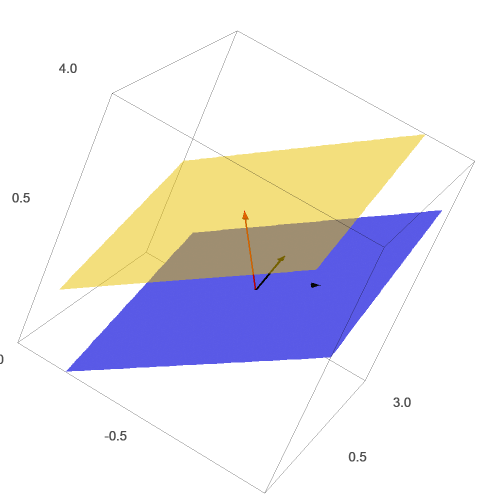
\includegraphics[width=1.25in]{images/solution_set}
			\end{center}
		\end{enumerate}
	\end{block}
\end{frame}
\begin{frame}{\fn}
\begin{block}{\textbf{Exercise \ref{translation} (Cont).}}
	\begin{center}
		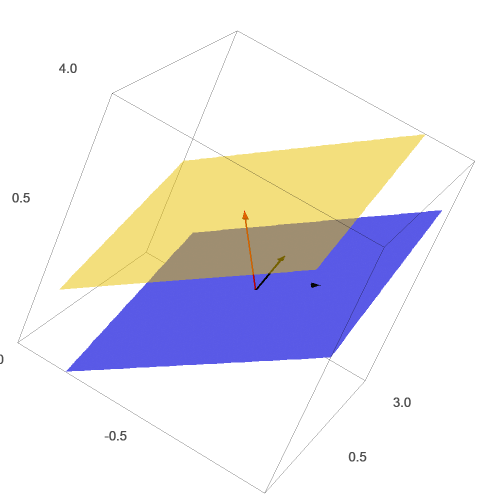
\includegraphics[width=1.25in]{images/solution_set}
	\end{center}
	\begin{enumerate}[label=(\alph*)]
		\item[(e)] Open
		{ \tiny\url{https://people.uwec.edu/westmr/teaching/1920-1-324/docs/sage4-6.txt}}
		and copy everything to \url{https://sagecell.sagemath.org/} so you can move/rotate the picture yourself.
	\end{enumerate}
\end{block}
\end{frame}
%\begin{frame}{\fn}
%	\begin{exercise}\label{nonhomogeneous}
%		Consider the system:
%			\[\begin{array}{rcrcrcr}
%				x&+&3y&-&3z&=&3\\
%				-2x&+&y&+&2z&=&-3\\
%				&&y&-&z&=&0\\
%				&&3y&-&2z&=&1
%			\end{array}\]
%		\begin{enumerate}[label=(\alph*)]
%			\item Determine whether the system is consistent.
%			\item If the system is consistent, write the solution in the form $\vec x=\vec x_p+\vec x_h$, where $\vec x_p$ is a particular solution of $A\vec x=\vec b$ and $\vec x_h$ is a solution of $A\vec x=\vec 0$.
%		\end{enumerate}
%	\end{exercise}
%\end{frame}
\begin{frame}{\fn}
	\begin{statementblock}{Theorem 4.19}
		The system $A\vec x=\vec b$ is consistent if and only if $\vec b$ is in the column space of $A$.
	\end{statementblock}
	\begin{proof}
		Let $A=\begin{bmatrix}\vec a_1&\vec a_2&\cdots & \vec a_n\end{bmatrix}$ where $\vec a_j$ represents the $j$-th column of $A$.  Notice that
			\[A\vec x=\begin{bmatrix}\vec a_1&\vec a_2&\cdots & \vec a_n\end{bmatrix}\begin{bmatrix}
			x_1\\x_2\\\vdots\\x_n
			\end{bmatrix}=x_1\vec a_1+x_2\vec a_2+\cdots+x_n\vec a_n.\]
			Therefore $A\vec x=\vec b$ if and only if $\vec b=x_1\vec a_1+x_2\vec a_2+\cdots+x_n\vec a_n$ is a linear combination of the columns of $A$.
	\end{proof}
\end{frame}

\begin{frame}{\fn}
	\begin{exercise}
		The system, $A\vec{x}=\vec{b}$ with
		
		\[A=\begin{bmatrix}1&3&10\\-2&7&32\\-1&3&14\\1&1&2\end{bmatrix}
		\text{ and }
		\vec b=\begin{bmatrix}
		18\\29\\12\\8
		\end{bmatrix}
		\]
		is consistent.
		Thus Theorem 4.19 says that $\vec b$ can be written as a linear combination of the columns of $A$.  Find such a combination. 
		
		Hint: Row reduce the augmented matrix $[A|\vec{b}]$.  The entries in the last column will indicate which values to use.
	\end{exercise}
\end{frame}
\begin{frame}{\fn}
	\begin{exercise}
		The dimension of the row space of a $5\times 3$ matrix $A$ is 2.
		\begin{enumerate}[label=(\alph*)]
			\item What is the dimension of the column space of $A$?
			\item What is the rank of $A$?
			\item What is the nullity of $A$?
			\item What is the dimension of the solution space of the homogeneous system $A\vec x=\vec 0$?
		\end{enumerate}
	\end{exercise}
\end{frame}
\end{document}

